\section{Introduction} 

Responses to the online survey questions allowed us to generate tacit and explicit knowledge sharing networks for each open innovation partnership. These networks represent empirical or observed reality in our critical realist study. Table \ref{tab:original_propositions} lists the seven propositions developed in Chapter \ref{chp:lit_review}. Together, the propositions represent an a priori causal framework for tacit knowledge exchange in open innovation (the first step in our critical realist analytical process). The propositions are broad in scope and are not subject to testing. They serve to guide our exploration of the social mechanisms that underpin tacit knowledge sharing. The apriori causal framework assumes that individuals choose to share or seek out tacit knowledge to satisfy an innate need for self-determination, be this greater personal autonomy, wanting to become more competent, demonstrating their worth, or connecting with others. Factors such as subjective and behavioural norms, real or perceived boundaries, rules of engagement, and trust and power relations are likely to influence tacit knowledge exchanges. One expects brokers to play a crucial role in helping individuals connect with others, overcome boundaries, build trust, manage power relations, and, importantly, deliver successful collective outcomes in open innovation projects. \medskip

\begin{table}[hbt!]
\centering
\caption{Original list of propositions.}
\label{tab:original_propositions}
\resizebox{\textwidth}{!}{%
\begin{tabular}{@{}c p{12cm}@{}}
\toprule
Proposition & Statement \\ \midrule
1a & Open innovation requires practitioners to connect across organisational and disciplinary boundaries so that they can transfer and apply their know-how and know-what in novel ways. \\
1b & Reducing cognitive distance between open innovation partners requires significant social interaction to support learning and the application of knowledge in practice. \\
2 & Successful open innovation requires deliberate brokerage actions that lead to network closure. \\
3a & Formal structures inhibit tacit knowledge exchange in open innovation partnerships. \\
3b & Innate needs and subjective norms moderate individual willingness to seek out or share tacit knowledge. \\
4a & Reciprocity and closure in tacit knowledge exchange networks indicate high levels of trust in open innovation partnerships. \\
4b & Who people choose to empower with their know-how depends on how much they trust the receiver to use their know-how in mutually beneficial ways. \\ \bottomrule
\end{tabular}%
}
\end{table}

We modelled specific network configurations related to our a priori causal framework. Model parameters were defined using the logic of deduction. One set of models tested propositions about the role of motivation, trust, and power in explicit and tacit knowledge networks. Another set of models examined the mix of broker roles in the networks. We then applied the logic of retroduction to code semi-structured interview transcripts. Retroduction uses both inductive and deductive logic, as well as insights or hunches. It involves thinking through what causal powers might be at work to produce our observed reality \citep{jagosh2020retroductive}. The interview transcripts shed light on how unobserved reality influences tie formation in the different tacit knowledge provider networks (the second step in our critical realist analytical process). \medskip

This chapter now applies the logic of retrodiction to create a cross-case causal framework. Retrodiction involves merging the causal frameworks for each case to explain differences and to create an a posteriori framework that offers a more general explanation of the mechanisms involved in tacit knowledge sharing \citep{welch2011theorising,mcavoy2018critical}. The chapter begins by briefly reminding us why agency versus structure matters in open innovation. It then describes how agency and structure influenced tacit knowledge sharing in each case before generalising these influences through cross-case analysis. Following the critical realist process outlined by \citet{mcavoy2018critical}, the chapter closes with a set of refined propositions based on the findings of this study. The refined propositions capture the learnings from this study and can form the basis for follow-up research.

\section{Why agency versus structure matters}

Recall from Chapter \ref{chp:intro} that tacit knowledge is the \enquote{unwritten, unspoken, and hidden vast storehouse of knowledge held by practically every normal human being, based on his or her emotions, experiences, insights, intuition, observations, and internalised information} \citep{kreutz2014catalyzing}. Tacit knowledge is not transferred, but interpreted within a specific context \citep{nonaka1994dynamic,duguid2005art,marabelli2014knowing,zhang2020extended}. As mentioned at the beginning of the thesis, the open innovation literature has paid scant attention to tacit knowledge. Managing tacit knowledge flows across organisational boundaries is not easy. Tacit knowledge is a tremendous source of personal power and nobody will surrender their tacit knowledge if this will potentially compromise them. Sharing tacit knowledge takes significant effort and people need to be sufficiently motivated to either demonstrate their know-how or observe how others enact their know-how in practice \citep{gagne2009model}. Because tacit knowledge exchange involves effort and is primarily an act of free will, the thesis argues that human agency lies at the heart of tacit knowledge sharing. \medskip

The concept of agency can be traced back to \citet{parsons1937structure} who posits that a strong desire to satisfy innate needs drives human action. He goes on to suggest that subjective or social norms influence individual choices. The relationship between agency and structure is central to \citeauthor{giddens1984constitution}'s \citeyearpar{giddens1984constitution} theory of structuration. He characterises the power of agents to intervene as a transformative capacity and refers to the \enquote{duality of structure} where structure not only constrains agency but is also transformed by agency. Although scholars accept that structure and agency are deeply entangled, there is still some controversy around which is more important. For example, \citet{archer1998critical} question \citeauthor{giddens1984constitution}'s \citeyearpar{giddens1984constitution} separation of agency and structure. They assert it is impossible to unpick structure and agency analytically because structure always precedes agency and both structure and agency operate on different timescales. \citet{loyal2001agency} believe that \citeauthor{parsons1937structure}'s \citeyearpar{parsons1937structure} and \citeauthor{giddens1984constitution}'s \citeyearpar{giddens1984constitution} view of agency is too deterministic. They object to the predictability of human actions based on individual wants, desires, or needs. \citet{loyal2001agency} think human actions are either chosen or caused and suggest that both individuals and social structures have distinctive causal powers that interact to determine social events. \citet{loyal2001agency} embrace a critical realist view of agency versus structure, one that recognises the complex nature of the real world. \citet{giddens1984constitution} has a much narrower view of agency versus structure. As stated earlier in this thesis, finding the right balance between structure and agency is a challenge in open innovation. Too much structure may inhibit individual willingness to share tacit knowledge or contribute ideas \citep{davis2010agency}. Conversely, too little structure can make goals less clear, leading to unsatisfactory open innovation outcomes \citep{lam2000tacit}. This study employs \citeauthor{loyal2001agency}'s \citeyearpar{loyal2001agency} agency model to assess how different causal mechanisms interact to shape tacit knowledge sharing ties in our three open innovation partnerships (Figure \ref{fig:agency_structure4}). 

\begin{figure}[hbt!]
    \centering
    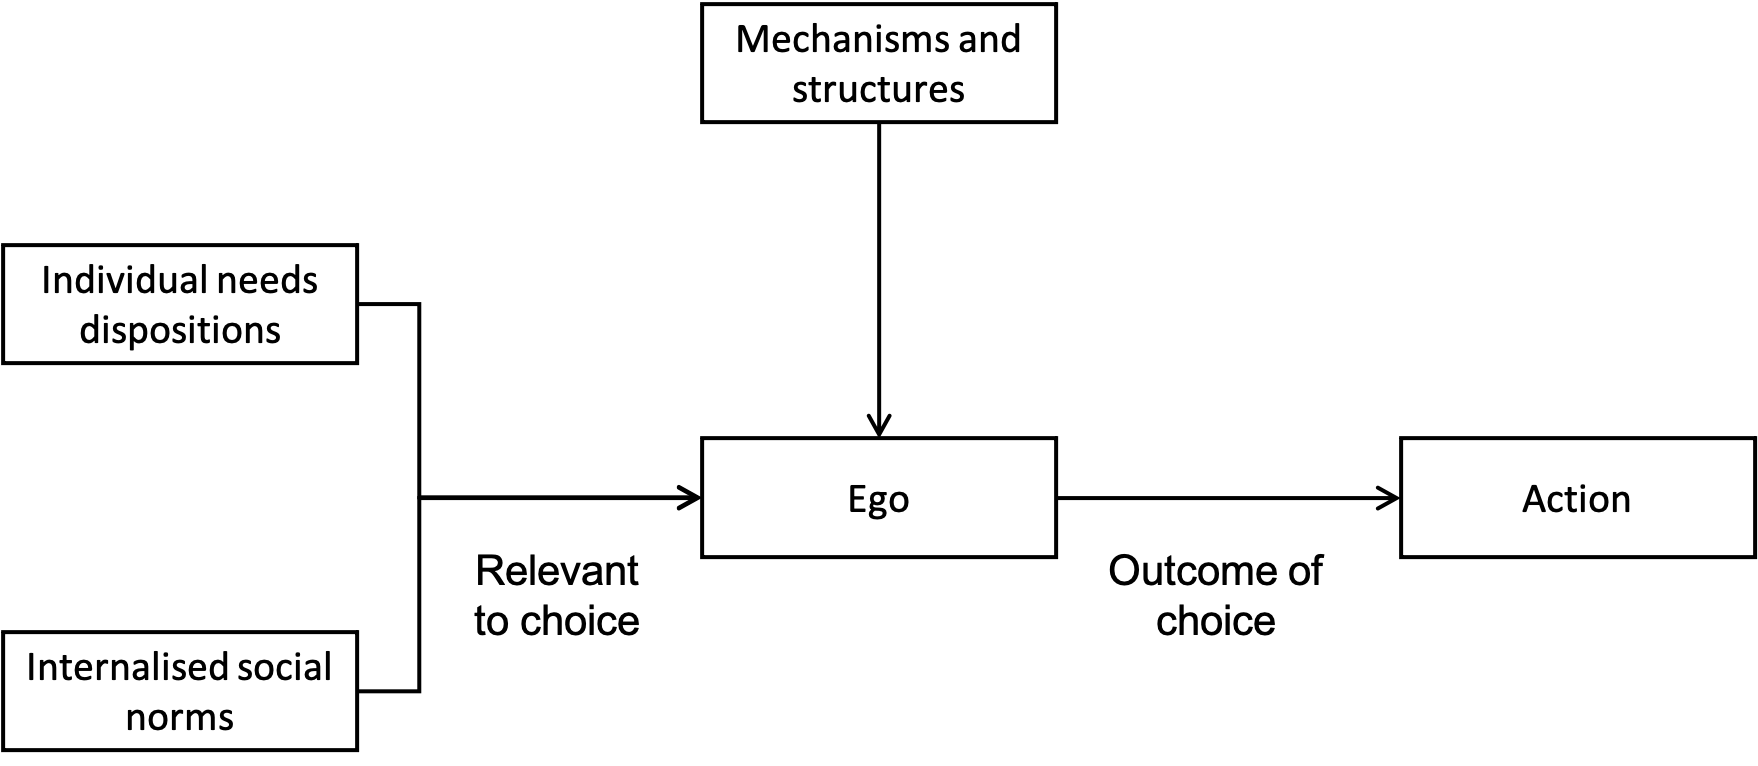
\includegraphics[width = \textwidth]{Images/agency_structure_loyal.png}
    \caption[]{Critical realist perspective of agency versus structure. Agency is about making intentional choices. Choices may be tempered by internalised social norms and social reality more broadly \citep{loyal2001agency}.}
    \label{fig:agency_structure4}
\end{figure}

\section{Emergence of tacit knowledge sharing ties in each case}

This section considers the causal mechanisms that appear to drive or inhibit the emergence of tacit knowledge sharing ties in light of the results presented in Chapters 6 and 7. The reader may need to refer to Figures \ref{fig:network_case_1} to \ref{fig:network_case_3}, Tables \ref{tab:ergm_1} to \ref{tab:ergm_3}, and Tables \ref{tab:case_1_codes} to \ref{tab:case_3_codes} for context.

\subsection{Case 1}

Case 1 was at an early stage at the time of data collection and the tacit knowledge provider network was only just beginning to emerge. The tacit knowledge provider network was notably much sparser than the explicit knowledge provider network. The semi-structured interviews revealed that university participants could not interact directly with refrigerated freight companies. The general manager driving the cold chain initiative did not want the university participants to complicate his commercial relationships with the freight companies and used his power over others or authority to limit interactions. He operated as a gatekeeper, believing he was the best person to translate technical information. His actions limited agency vital for the sharing of know-how. \medskip

The ERGM analysis shows that participants who are either autonomously motivated or open to experience are more likely to seek out tacit knowledge. Becoming more competent, improving practices, and performing meaningful work featured strongly in the semi-structured interviews. Modelling indicates that tacit knowledge is shared in local network neighbourhoods (i.e. a local community of practice). There is also a strong correlation between cognition-based trust and tacit knowledge sharing ties. Past studies indicate that trust features strongly in tacit knowledge exchanges \citep[e.g.][]{kaser2001knowledge,lin2007share,zhang2016critical}. The semi-structured interviews revealed that participants were less inclined to share their know-how with others they did not trust, especially if this would compromise their organisation's commercial interests. Tacit knowledge exchanges were more likely to occur between people in close geographic proximity. \medskip

Analysis of broker roles shows representative brokers feature prominently in the tacit knowledge provider network indicating a significant number of participants were inclined to share their know-how with third parties. One good example of this is the cold loading dock advice provided by the main refrigerated freight company to the leafy vegetable grower (e.g. space needed to back up trucks, concreting the apron, height of loading bay, type of doors). Another example is the operational knowledge provided by the general manager to the university participants (e.g. how produce is harvested, washed, packaged, and dispatched to customers). The interviews also reveal that some participants withheld knowledge from other partners because they did not think they would understand it, further limiting the development of the tacit knowledge provider network. \medskip

Summing up, the participants in this case were motivated to acquire tacit knowledge. Analysis of broker roles shows that participants were willing to share their know-how with third parties. However, their ability to connect with others with relevant know-how was affected by restrictions imposed by the general manager and geographic separation. Trust was an essential prerequisite for tacit knowledge sharing. The sparseness of the tacit knowledge provider network can be attributed to the early stage the project was at (relationships were still forming), but also due to gatekeeping by the general manager (an example of structure limiting agency in open innovation).

\subsection{Case 2}

Case 2 was winding down at the time of data collection. By this stage, the tacit knowledge provider network was fully formed. The objective of getting a herd of 600 cows to engage in voluntary milking had been achieved, and the partnership was past peak tacit knowledge sharing. Modelling of the tacit knowledge provider network shows a significant and positive path closure effect combined with a significant and negative multiple connectivity (broker) effect, a sign of strong collaboration. Experienced participants were also happy to share their know-how with less-experienced others (indicated by a significant and positive work experience sender effect). The pasture specialist sharing his knowledge of pasture management with the dairy farmer is an example of this. \medskip

The dairy farmer was driven to master the milking robot technology, often putting in 100 hour weeks to ensure things were working correctly. He wanted to prove to the dairy industry that voluntary milking could work. Likewise, the company responsible for installing and maintaining the milking robots was also keen to master this technology. Their ambition was to become an industry leader in selling and servicing milking robots. The engineers who designed the milking robots were unfamiliar with the voluntary milking concept and flew across the world to witness issues on the dairy farm firsthand. Not only does this show commitment to learning, but it also may explain why geographic separation was not a significant issue like it was in Case 1 and Case 3. The semi-structured interviews highlighted the importance of investing in relationships to allow open and honest discussion. Such openness built trust and made it easier to align thinking and experiment with different approaches. Experimentation helped participants gain additional know-how. The main partners were very committed and shared in the decision-making. \medskip

In summary, the partnership had successfully achieved its primary objective. Much of the success is due to everyone having a clear understanding of what was needed and demonstrating strong commitment. Focusing on relationships and engaging in mutual learning also helped deliver success. No single partner dominated proceedings, which allowed everyone feel they had a role to play. The way the partnership was structured and managed helped promote individual agency. Participants were sufficiently empowered and were able to choose who they exchanged tacit knowledge with. 

\subsection{Case 3}

Case 3 was at an early stage at the time of data collection, and the tacit knowledge provider network was still emerging. Unlike Case 1, tacit and explicit knowledge exchanges were more or less evenly balanced. Tacit knowledge tended to come from a few central actors (indicated by a significant and positive activity spread effect). Brokers usually feature more prominently in new partnerships, and this was evident in this case. Analysis of broker roles shows the gatekeeper and representative roles featured strongly in tacit knowledge exchanges. Brokers had a significant influence over tacit knowledge flows. \medskip   

Contrary to what the literature suggests \citep[e.g.][]{osterloh2000motivation,kaser2001knowledge,obrenovic2020enjoyment}, the network analysis reveals that participants felt obliged to share their tacit knowledge. One can expect participants not familiar with bee-tracking technology to be pushing others for information on how the technology works. Participants were strongly encouraged to capture their learning on the wiki. However, not many were inclined to do so. Nevertheless, extrinsically motivated participants were less likely to receive tacit knowledge. As with the other two cases, autonomously motivated participants are more likely to seek tacit knowledge from others. Participants who identified strongly with their workgroup were less inclined to share their tacit knowledge with others. However, mutual or reciprocal sharing of tacit knowledge among partners (and perhaps brokers, more specifically) was significant. As with the other cases, participants were more likely to share their tacit knowledge with others they trusted. \medskip

The semi-structured interviews revealed that the partnership was grappling with several issues. Personality differences, professional jealousy, organisational politics, and participants acting in their self-interest hindered collaboration. The dissemination of knowledge was centrally coordinated, which limited partner interaction. Little consideration appears to have been given to the role of tacit knowledge in the design of the open innovation partnership. The geographic spread of partners, reliance on electronic communication, and language barriers made tacit knowledge sharing even more challenging. Moreover, the national research agency oversold the technology they provided, and when it did not work as expected, partners became frustrated and disillusioned. Funding constraints also limited what the partnership could achieve. The team members behind the initiative felt that many of the participating scientists were not very committed and too conservative in how they did research. They also felt that some scientists were dismissive of the technological challenges confronting them. A senior manager at the national research agency attributed many of the problems to poor leadership. However, one participant felt that organisational politics and participants with large egos contributed to many of the issues. Case 3 had a relative high proportion of participants with doctoral level qualifications (see Figure \ref{fig:demographics}). One expects highly qualified people to be empowered and able to operate with a significant amount of autonomy \citep{goller2017human}. This case may be an example of participants having too much agency. \medskip

In summary, while many of the participants were excited about using new technology, not all the partners bought into the vision of a global partnership. There was no real commitment to achieving a common goal. Exchanging know-how was challenging, given the tension between partners, lack of face-to-face interaction, language barriers, and competing research agendas. On the one hand, too much structure limited agency, and on the other hand, too little structure in terms of commitment, leadership and shared objectives led to participants to pursue their own agendas without much regard for the partnership (too much agency).

\section{Similarities between cases}

Although the three cases are very different in their stage, open innovation archetype, and industry context, they share a few similarities. This section focuses on what is similar among the three cases. \medskip

Both Case 1 and Case 3 were at an early stage and one would expect tacit knowledge sharing ties to be less developed than those in the much more mature Case 2. The main proponents in both Case 1 and Case 3 occupied a very central position in their respective tacit knowledge provider networks. They controlled partner interactions, thereby limiting agency. Neither proponent fully appreciated the importance of tacit knowledge for open innovation. Case 2 was different in that partners worked together to define the goal of the partnership. Integrating diverse know-how was essential for success. Nobody had privileged access to know-how, and agency thrived as a consequence. \medskip

Regarding the modelling results, we have significant path closure in the Case 1 and Case 2 but not the Case 3 tacit knowledge provider networks. The combined tacit knowledge provider network also has significant path closure (Table \ref{tab:case_2_codes}). Path or transitive closure occurs when all the members of a triad become connected, forming a triangle \citep{yin2020measuring}. It indicates tacit knowledge sharing occurs in small groups. The modelling confirms what past studies have found, namely the sharing of tacit knowledge is primarily a social act \citep{nonaka1994dynamic,kaser2001knowledge,zhang2016critical}. The combined tacit knowledge provider network modelling shows a significant and positive effect for activity spread. We only see this effect in Case 3. Essentially, the combined network analysis indicates that, in general, tacit knowledge is more likely to come from a few select actors. Again, there is a significant and positive effect for education level difference in the combined tacit knowledge provider network but not in case-specific tacit knowledge provider networks. This effect indicates there is a general heterophily effect for education level. Other factors probably mask this effect in individual cases. \medskip

The modelling is unambiguous for autonomous motivation being a good predictor of tacit knowledge-seeking behaviour. The same applies to the correlation between tacit knowledge sharing and cognition-based trust ties. Cognition-based trust appears to be important for sharing tacit knowledge. These findings are consistent with those reported by \citet{holste2010trust} and \citet{gubbins2021delineating}. \medskip

The modelling of broker roles in the tacit knowledge networks shows that brokerage differs considerably between the cases and that one can characterise open innovation partnerships in terms of brokerage patterns alone. One cannot compare the two sets of modelling results. The models examining broker roles looked at purely structural effects only. Nonetheless, the modelling of broker roles appears to be picking up some subtleties in how tacit knowledge is being exchanged. ERGM parameter estimates are usually seen to represent an average social process operating across the entire graph. The ERGM analysis of broker roles suggests that such generalisation misses important nuance. Broker roles represent distinct triadic structures distinguished by group membership and are likely to be subsuming other more general triadic structures \citep{gould1989structures}. Modelling of broker roles may be providing a more nuanced and precise explanation of the structure of inter-organisational knowledge networks. \medskip

We see some similarities between cases in the qualitative coding results. Becoming more competent and performing meaningful work is common to all three cases and helps explain why autonomous motivation drives tacit knowledge seeking. Many of the codes are common to only two of the three cases. For instance, in Case 1 and Case 3, we see that some participants maintain narrow perspectives, demonstrate superior attitudes, and communicate poorly. The need to tap external expertise is common to Case 1 and Case 3. Participants in Case 1 and Case 2 emphasised the importance of maintaining good relations to allow open and honest discussions. Cases 2 and 3 involved participants based in different parts of the world, and unsurprisingly, dealing with the tyranny of distance was an issue for both. Overall, there are more dissimilar than similar codes. The dissimilarity emphasises that each case is unique and that one has to be cautious when generalising results from individual case studies. Indeed, ERGM as an approach to modelling social network data does frame a particular network under study as a unique case in itself, with the model results comparing the network in this particular social context with other ways the same network could be arranged, not  with some generalised \enquote{norm} from a collection of social contexts. 

\section{Revised causal framework}

The initial set of propositions was evaluated using a combination of exponential random graph modelling and analysis of semi-structured interviews. This section reviews the initial set propositions in light of the evidence from the modelling and analysis of semi-structured interviews. It then presents a revised set of propositions that represent our a posteriori causal framework. 

\subsection{Evidence supporting the initial set of propositions}

\subsubsection{Proposition 1a}

Proposition 1a states that \enquote{open innovation requires practitioners to connect across real and perceived boundaries to apply their know-how in novel ways}. One may expect to see evidence of path closure, employer mismatch, and employer mismatch reciprocity in the ERGM analysis of tacit knowledge provider networks. Path closure is a sign that people with know-how are working together. Employer mismatch indicates participants are connecting across organisational boundaries, whereas employer mismatch reciprocity points to mutual tacit knowledge sharing across organisational boundaries. The qualitative results should reveal what participants consider to be real and perceived boundaries affecting tacit knowledge exchanges. \medskip 

The evidence collected in this study provides insufficient support for Proposition 1a. Path closure is significant in both the combined tacit knowledge provider network and two of the case-specific tacit knowledge provider networks. Aside from Case 3, we do not see significant employer mismatch or employer mismatch reciprocity. On the contrary, we see a significant employer match effect in the combined tacit knowledge provider network. Despite the evidence of strong collaboration in Case 2, it still has a significant employer match effect. Participants are not connecting across organisational boundaries in a significant way. They prefer to share their know-how with work colleagues and not so much with external partners. Perhaps we need to think about connecting internal communities of practice instead of individual participants \citep{garrety2004integrating,venkitachalam2012tacit}. Thinking this way would shift emphasis from agency to brokerage and would have significant implications for open innovation project design \citep{wenger2000communities}. 

\subsubsection{Proposition 1b}

Proposition 1b states that \enquote{reducing the cognitive distance between open innovation partners requires significant social interaction to support learning and the application of knowledge in practice}. This study did not attempt to measure the cognitive distance between open innovation partners. However, we can measure social interaction and infer learning from our network data. More specifically, we would be looking for significant autonomous motivation receiver and employer mismatch reciprocity effects in our tacit and explicit knowledge provider networks. The autonomous motivation receiver effect would indicate a propensity for learning while employer mismatch reciprocity is a sign of mutual knowledge sharing across organisational boundaries, i.e. learning from one another. The semi-structured interview data should also yield information about the amount of learning happening in each partnership. \medskip

We do see significant autonomous motivation receiver effects in all the tacit knowledge provider networks. However, employer mismatch reciprocity was only significant in the Case 3 tacit knowledge provider network. The semi-structured interviews reveal that participants were motivated to learn, especially in Case 1 and Case 2. Proposition 1b is reasonably well-supported by the evidence. 

\subsubsection{Proposition 2}

Proposition 2 states that \enquote{successful open innovation requires deliberate brokerage actions that lead to network closure.}. We are looking for evidence of path closure in our network analysis and references to deliberate broker actions (brokerage performed with a clear outcome in mind) in the analysis of semi-structured interviews. As stated earlier, path closure is significant in all but the Case 3 tacit knowledge provider networks. Path closure is not significant in the case-specific explicit knowledge provider networks. However, we do see significant path closure in the combined explicit knowledge provider networks. \medskip

Evidence of deliberate brokerage is patchy. Brokerage does not feature strongly in the ERGM results for Case 2. This finding is not surprising given Case 2 had all but run its course. However, the qualitative analysis does reveal some examples of deliberate brokerage actions in Case 2. For instance, the dealer for the milking technology provider recruited the dairy farmer to trial voluntary milking. Another example is the local representative for the milking technology provider who helped broker connections between the dairy farmer and head-office personnel (both examples of tertius iungens brokerage). \medskip

Overall, the evidence suggests that participants in all three cases were reactive rather than proactive in their brokerage. Much of the literature considers brokerage to be transient. This is evident in our network analysis. Brokerage features more strongly in Case 1 and Case 3 that were both at an early stage, compared to Case 2, which was in its closing stages. \citet{grosser2019measuring} write about the need to engage in \enquote{sustained} tertius iungens brokerage in some coordination or project management role. This need is particularly important in open innovation to ensure the different parties are working effectively together. Tertius gaudens brokerage is expected to feature in partnerships where partners are wary of giving away too much information or knowledge spillover. We see circumstantial evidence for this in Case 1, where the general manager prevented the university researchers from engaging directly with his refrigerated freight providers. Although he did not want the researchers to complicate his relationship with the freight providers, it appears he was also concerned about knowledge spillover. \medskip

Proposition 2 ought to be amended to be more clear about the role of of tertius iungens brokerage for empowering participants and coordinating action. Tertius gaudens brokerage is also expected to feature more strongly in less open partnerships. Proposition 2 needs to be more explicit about organisational boundaries as well. 

\subsubsection{Proposition 3a}

Proposition 3a states that \enquote{formal structures inhibit tacit knowledge exchange in open innovation partnerships}. One would expect the modelling to show path closure and autonomous motivation sender or receiver effects to be under-represented, and the controlled motivation sender effect to be over-represented. The qualitative analysis of interview transcripts highlighted specific instances where structure may have inhibited tacit knowledge sharing. \medskip

The modelling shows path closure is over-represented in all but one of the tacit knowledge provider networks. There was no significant path closure in Case 3. All the tacit knowledge provider networks show a significant autonomous motivation receiver effect. As mentioned earlier, there is a significant and positive sender effect and a significant and negative receiver effect for controlled motivation in the Case 3 tacit knowledge network. The opposite effects suggest that people felt some pressure to share their tacit knowledge but not so much pressure to acquire tacit knowledge in Case 3. Essentially, the modelling suggests that formal structures did not inhibit tacit knowledge sharing in Case 1 or Case 2 but did in Case 3. \medskip

The qualitative analysis does provide some evidence of formal structure getting in the way of tacit knowledge sharing. In Case 1, university researchers were not allowed to engage directly with the freight companies. Participants from the freight companies had many years of cold-chain experience, and the university researchers were unable to tap into this experience. Formal structure did facilitate tacit knowledge sharing in Case 2. The milking technology provider's executive management approved sending engineers across the world to witness events on the dairy farm firsthand. The hub-and-spoke management model used in Case 3 prevented partners from engaging more directly with each other. \medskip

Evidence supporting Proposition 3a is mixed. There is some merit in combining Propositions 2 and 3a. Employing strategic brokerage to facilitate tacit knowledge sharing may be construed as an example of formal structure enabling agency. Combining Propositions 2 and 3a allows one to consider the positive and negative impacts of structure on human agency. 

\subsubsection{Proposition 3b}

Proposition 3b states that \enquote{Individual needs dispositions and internalised social norms moderate a person's willingness to seek out or share tacit knowledge}. Essentially we are looking for evidence concerning psychological needs of individual participants and their impact on group behaviour. Autonomous motivation, openness to experience, and social identity featured in the first set of ERGM models. The semi-structured interviews did ask questions about partner behaviour and attitudes. \medskip 

As reported earlier, the modelling shows a significant receiver effect for autonomous motivation in all the tacit knowledge networks. This effect indicates a propensity to seek out tacit knowledge interpreted as a desire to satisfy an innate need for competence, autonomy, or social connection. The modelling is able to discriminate between knowledge sharing and knowledge seeking behaviour and shows that knowledge seeking is dominant in all three partnerships. \medskip

We see a significant openness to experience receiver effect in Case 1. People receiving tacit knowledge in Case 1 tend to be more open. We also see a significant and negative identification-with-group sender effect in the Case 3 tacit knowledge provider network. People who do not identify strongly with their workgroup are more likely to share tacit knowledge with others in Case 3. Looking at social identity more broadly, participants appear to identify quite strongly with the partnership in Case 1 compared to Case 2 and Case 3 (see Table \ref{fig:psycho}). \medskip

The qualitative analysis reveals that participants from all three cases were motivated to perform meaningful work. Satisfying an innate need for competence was more apparent in Case 2 and Case 3. Some participants in Case 1 and Case 3 appeared to demonstrate a sense of superiority in relation to knowledge sharing. Two interviewees from Case 1 doubted the ability of freight companies to grasp thermodynamic principles. Some participants in Case 3 looked down on technologists and questioned the scientific credibility of the project leader driving the global initiative. The team behind the global initiative felt that some of the participating scientists were narrow-minded and risk-averse. Harbouring superior attitudes and being judgemental indicates a level of close-mindedness that is not conducive for tacit knowledge sharing. One participant from Case 3 remarked that egos were getting in the way of progress. Strong personalities are likely to negatively impact willingness to share or seek out tacit knowledge \citep{borges2012tacit}. In spite of all the tensions in Case 3, participants from Case 3 reported higher levels of agreeableness than the participants in Case 1 and Case 2 (Table \ref{fig:psycho}). Case 3 appears to have tested participants' ability to work across disciplinary and cultural boundaries. \medskip

The quantitative and qualitative evidence supports Proposition 3b. That said, there is merit in refining Proposition 3b to refer to specific needs and attitudes. 

\subsubsection{Proposition 4a}

Proposition 4a states that \enquote{reciprocity and closure in tacit knowledge exchange networks indicate high levels of trust in open innovation partnerships}. Whereas the modelling results indicate path closure is over-represented in each case's tacit knowledge network, reciprocity is not a significant effect in any of these networks. These effects are mirrored in the combined tacit knowledge network analysis. One exception is the significant and positive effect for employer mismatch reciprocity seen in Case 3. The modelling shows a significant and positive co-entrainment effect between tacit knowledge sharing and cognition-based trust. People are more likely to share their know-how with others they trust. The qualitative analysis indicates there is a high level of trust in Case 2. However, we do not see any significant reciprocal sharing of tacit knowledge in the network analysis. Reciprocity does not appear to be a reliable indicator of trust. Some of this may be explained by knowledge asymmetry. Participants seeking know-how from others may not have much know-how to give in return \citep{hahl2016knowledge,tell2017managing}. Proposition 4a needs to be modified to reflect this.

\subsubsection{Proposition 4b}

Proposition 4b states \enquote{whom people choose to empower with their know-how depends on how much they trust the receiver to use this know-how in mutually beneficial ways}. We need to rely on evidence from the qualitative analysis to assess this proposition. With Case 1, the leading freight company willingly advised the leafy vegetable grower on how to configure their loading docks. The freight company knew that sharing their know-how would strengthen relations with their primary customer and help the green leafy vegetable grower deliver products with a longer shelf life. The general manager driving the cold-chain initiative and sales manager from the temperature sensor provider stated they were reluctant to share their knowledge with others they did not fully trust. Both expressed concern about technology spillover to competitors. \medskip

Participants in Case 2 willingly shared their know-how to ensure the partnership succeeded in achieving its goal. The pasture specialist shared his know-how with the dairy farmer to ensure cows moved through the different grazing areas to the dairy. Likewise, scientists from the dairy research institute helped the dairy farmer design his grazing system to enable voluntary milking. The milking technology provider and their local dealer worked closely with the dairy farmer to iron out difficulties with robot technology. Everybody benefited from the knowledge sharing. Having a shared understanding and common goal did facilitate knowledge sharing. \medskip

The use of a wiki to capture information about the different experimental setups was an attempt to empower participants in Case 3. Unfortunately, the lead software engineer became increasingly responsible for maintaining the wiki. Not all the partners were that keen to share their experiences through a wiki. It appears many of the participants in Case 3 prioritised their needs ahead of those of the partnership. Scientists did not want others to claim credit for the work they were doing. They played their cards close to their chest because they did not trust other scientists. Overall, we see evidence from all three cases supporting Proposition 4b. People share their know-how if they perceive it will be beneficial for them or their employer \citep{liu2021more}.

\subsection{Revised propositions}

A case-based study allows one to compare and contrast different cases to come up with a more generalised causal framework \citep{welch2011theorising}. We examined how the original set of propositions stacked up in each of our three cases. The evidence shows that support for our propositions is mixed and that some refinement of these is warranted. The refined propositions presented below capture the learnings from this study and can form the basis for follow-up research. \medskip

\begin{sidewaystable}[hbtp]
\caption{Revised propositions.}
\label{tab:new_propositions}
\resizebox{\textwidth}{!}{%       
\begin{tabular}{@{}cp{12cm}l@{}}
\toprule
Revised proposition & Statement & Notes \\ \midrule
1 & Open innovation requires internal communities of practice to connect across boundaries to transfer and apply their know-how in novel ways. Brokerage is essential for connecting these communities of practice but becomes less critical as these communities become increasingly inter-connected. & Merger of Proposition 1a and 2 \\
2 & Autonomous motivation is a reliable predictor of knowledge-seeking behaviour in open innovation partnerships. People seek out knowledge to improve their level of self-determination and satisfy a desire to perform meaningful work. & Combines elements of Propositions 1b and 3b \\
3 & Participants who demonstrate superior or close-minded attitudes compromise their absorptive capacity and that of their employer. They are less inclined to learn about things outside their domain of expertise and undermine efforts to bring diverse know-how and knowledge together. & Includes elements of Proposition 3b \\
4 & A successful open innovation partnership builds cognition-based trust by investing in relationships that allow open and honest discussions. Path closure in tacit knowledge provider networks is a good indicator of cognition-based trust. & Updated Proposition 4a \\
5 & The extent to which participants empower others with their know-how in an open innovation partnership depends on how much they consciously trust them to use it mutually beneficial ways. & Updated Proposition 4b  \\ \bottomrule
\end{tabular}
}
\end{sidewaystable}

Table \ref{tab:new_propositions} presents an updated set of propositions based on the modelling results and analysis of semi-structured interviews. Propositions 1a and 2 have been merged into a revised proposition: \bigskip

\begin{tcolorbox}
\textit{\textbf{Revised proposition 1:} Open innovation requires internal communities of practice to connect across boundaries to transfer and apply their know-how in novel ways. Brokerage is essential for connecting these communities of practice but becomes less critical as these communities become increasingly inter-connected.} 
\end{tcolorbox}

This revised proposition advocates a community of communities approach, setting up an overarching community of practice to achieve a specific open innovation outcome \citep{palla2005uncovering, west2008getting, sytch2014exploring, dumbach2014establishing}. Members of internal communities of practice tend to develop mindsets and practices that reflect their professional training and experience \citep{garrety2004integrating,wenger2011communities}. The open innovation challenge is to overcome communication barriers between communities with quite different skills, languages, expectations and assumptions \citep{fleming2007brokerage,chesbrough2012open}. Effective brokerage requires a good understanding of how each community of practice operates and the development of a shared goal that each community buys into \citep{garrety2004integrating,adler2008perspective,hargadon2014brokerage,kwon2020network}. The farm systems specialist (Participant 9/2) and research project leader (Participant 9/2) demonstrated this to good effect. Tertius iungens brokerage is particularly well-suited to this situation \citep{obstfeld2014brokerage, quintane2016brokers, grosser2019measuring}. \medskip

The need for tertius iungens brokerage lessens as communities of practice become increasingly inter-connected (indicated by the emergence of heterophily, e.g. employer or field of research mismatch effects). To properly gauge open innovation and brokerage performance, one would need to measure knowledge sharing relations at both intra-organisational and inter-organisational levels \citep{jasny2015two}. \medskip

Proposition 1b refers to \enquote{reducing cognitive distance}. This proposition would benefit from re-framing. The term \enquote{cognitive distance} is loosely defined by \citet{nooteboom2000learning}. He refers to cognitive distance as a difference in cognitive function or learning capacity. The capacity to learn from partners is difficult to quantify. We may infer that learning is happening through social interaction measured in terms of network density, path closure, and reciprocity \citep{reagans2003network, marsden2012reflections, phelps2012knowledge}. It is also possible to infer learning orientation from autonomous motivation receiver effects, an indicator of knowledge seeking behaviour \citep{gagne2009model,gubbins2021delineating}. One can create a more robust proposition by combining elements of Proposition 1b and Proposition 3b: \bigskip

\begin{tcolorbox}
\textit{\textbf{Revised proposition 2:} Autonomous motivation is a reliable predictor of knowledge-seeking behaviour in open innovation partnerships. People seek out knowledge to improve their level of self-determination and satisfy an innate need to perform meaningful work.}
\end{tcolorbox}

Proposition 3b refers to internalised social norms moderating knowledge sharing or seeking behaviour. The semi-structured interviews revealed that participants with superior attitudes or those who maintain a narrow perspective were less inclined to share knowledge or learn from others. Proposition 3b can be modified to reflect this: \bigskip

\begin{tcolorbox}
\textit{\textbf{Revised proposition 3:} Participants who demonstrate superior or close-minded attitudes compromise their absorptive capacity and that of their employer. They are less inclined to pay attention to learn about things outside their domain of expertise and undermine efforts to bring diverse know-how and knowledge together.}
\end{tcolorbox}

This revised proposition considers absorptive capacity at both the individual and organisational levels. Learning is vital for reducing the cognitive distance between organisations exchanging knowledge or co-creating new knowledge \citep{nooteboom2000learning}. Employees who do not pay attention to, or who are not open to learning about, things outside their domain of expertise not only limit their absorptive capacity but that of their organisation as well \citep{yildiz2019fosters}. They are also less likely to participate in a broader community of practice in which participants want to apply know-how and know-what in novel ways. \medskip

Trust is the measure of belief that a given entity will act as one expects \citep{richters2011trust}. Humans will base their trust decisions on arbitrary criteria since there is no formal consensus on how to evaluate trust. One measure of trust is transitive or path closure in social networks \citep{coleman1988social,burt2001structural}. This measure works on the principle that if A trusts B and B trusts C, then A is inclined to trust C (also known as the \enquote{friend-of-a-friend} or \enquote{web-of-trust} principle). Two cases have significant path closure in their tacit knowledge provider networks (Case 1 and Case 2). There is a significant dyadic covariate effect between tacit knowledge sharing ties and cognition-based trust ties in all three cases. Thus, path closure in tacit knowledge provider networks is an indicator of trust \citep{sherchan2013survey}. The importance of having good relations that allow open and honest discussions features strongly in the qualitative analysis of Case 1 and Case 2. Both these cases also highlighted the importance of showing commitment. Case 3 is the exception here in that there was no significant path closure in the tacit knowledge provider network. The qualitative analysis highlighted a trust deficit. Moreover, strained relations did not allow open and honest discussions. Based on this evidence, we can re-frame Proposition 4a as follows: \bigskip

\begin{tcolorbox}
\textit{\textbf{Revised proposition 4:} A successful open innovation partnership builds cognition-based trust by investing in relationships that allow open and honest discussions. Path closure in tacit knowledge provider networks is a good indicator of trust.}
\end{tcolorbox}

The analysis of the semi-structured interviews did indicate that cognition-based trust features strongly in tacit knowledge sharing decisions. Proposition 4b is supported but can be revised to refer to open innovation more specifically: \bigskip

\begin{tcolorbox}
\textit{\textbf{Revised proposition 5:} The extent to which participants empower others with their know-how in an open innovation partnership depends on how much they consciously trust them to use it mutually beneficial ways.}
\end{tcolorbox}

We can qualify \citeauthor{loyal2001agency}'s \citeyearpar{loyal2001agency} agency model in terms of the revised propositions. The qualified model represents our a posteriori causal framework for tacit knowledge in open innovation. It assumes tacit knowledge resides in various communities of practice that exist within partner organisations. Individuals are primarily motivated to seek out tacit knowledge to improve their level of self-determination. However, individuals who are close-minded or consider themselves superior are less likely to connect with external communities of practice. Such attitudes undermine open innovation. The ability to tap external communities of practice is affected by several mechanisms that may include real or perceived boundaries and power and trust relations. Individuals are more likely to share their tacit knowledge if this delivers some benefit to them. Successful open innovation requires partners to invest in relationships that facilitate open and honest discussions. Brokers have a crucial role to play in connecting different communities of practice, especially in the early stages of open innovation. \medskip

\section{Chapter summary}

The propositions developed in Chapter 2 served as a theoretical starting point for our critical realist examination of tacit knowledge sharing in open innovation. Chapter 5 used social network analysis to (a) measure the structure of tacit and explicit knowledge sharing ties and (b) assess which personal attributes are likely to influence the formation of tacit and explicit knowledge ties in each case. The propositions informed which parameters to include in our network analysis. Results from the social network analysis represent our observed reality in our critical realist approach. Chapter 6 used semi-structured interviews to gain insight into each case's context, our unobserved or actual reality. The propositions helped us unpack the causal frameworks for each case. \medskip

This chapter used the logic of retrodiction to compare and contrast the quantitative and qualitative results presented in Chapters 5 and 6. Retrodiction involves merging the causal frameworks for each case to explain differences and to create an a posteriori framework that offers a more general explanation of the mechanisms involved in tacit knowledge sharing \citep{welch2011theorising,mcavoy2018critical}. The quantitative and qualitative results provide a \enquote{reality check} for our propositions. We revised our propositions in light of the evidence collected in this study. The revised propositions are evidence-based and thus provide a more credible a posteriori causal framework based on \citeauthor{loyal2001agency}'s \citeyearpar{loyal2001agency} agency model that can inform open innovation management practices with greater confidence. \medskip

The next and concluding chapter summarises what we have learnt about the tacit dimension of open innovation. This summary describes the main findings of this study and the implications of these for management. It outlines the main research contributions of this study before wrapping up with a brief discussion of study limitations and recommendations for future research.